\def\figpath{tex/4_Konstantstromquelle/pictures}
\graphicspath{{tex/4_Konstantstromquelle/pictures/}}

\chapter{Konstantstromquelle}
In Kapitel 4 wird die Auslegung einer Konstantstromquelle, welche mittels Bipolartransistoren realisiert wird, behandelt. Im folgenden wird auf die Berechnung, die Simulation und das Temperaturverhalten der Schaltung eingegangen. 

\section{Wahl der Stromquellenschaltung und Auslegung der Widerstände}
Für die zu untersuchende Stromquelle wird die Schaltung eines einfachen Stromspiegels gewählt, siehe Abb. \ref{fig_Kap4_01:Stromspiegel01}. 

\begin{figure}[H]
	\centering
	\def\svgwidth{0.5\textwidth}
	\input{\figpath/EinfacherStromspiegel.pdf_tex}
	\caption{Einfache Stromspiegelschaltung} 
	\label{fig_Kap4_01:Stromspiegel01} 
\end{figure}

Die Transistoren $T_1$ und $T_2$ werden baugleich gewählt (jeweils Typ BC547B), womit auch 
\begin{equation}
    B_1 = B_2 = B
\end{equation}
gelten soll. 

Des weiteren gilt für den Kollektorstrom an einem npn-Bipolartransistor

\begin{equation}
    \label{glgn_transist}
    I_C = I_S \left(e^{\frac{U_{BE}}{U_T}} - 1 \right) .
\end{equation}

Für Masche I aus Abb. \ref{fig_Kap4_01:Stromspiegel01} gilt

\begin{equation}
    \text{MI: } U_{BE,1} + I_{C,1}\left( 1 + \frac{1}{B}\right)R_{E,1} = U_{BE,2} + I_{C,2}\left( 1 + \frac{1}{B}\right)R_{E,2} .
\end{equation}

Wählt man beide Emitterwiderstände gleich groß (jedoch $\nequ 0 $), so ergibt sich die Gleichung

\begin{equation}
    U_{BE,1} + I_S \left(e^{\frac{U_{BE,1}}{U_T}} - 1 \right)\left( 1 + \frac{1}{B}\right)R_E = U_{BE,2} + I_S \left(e^{\frac{U_{BE,2}}{U_T}} - 1 \right)\left( 1 + \frac{1}{B}\right)R_E .
    \label{glng_transzend}
\end{equation}

Es ist naheliegend, dass sich durch den symmetrischen Schaltungsaufbau als Lösung der transzendenten Gleichung \ref{glng_transzend} wiederum gleich große Basis-Emitterspannungen einstellen werden, 

\begin{equation}
    U_{BE,1} = U_{BE,2} .
\end{equation}

Aus Gleichung \ref{glgn_transist} folg somit
\begin{equation}
    I_{C,1} = I_{C,2} = I_C \quad \Rightarrow \quad I_{B,1} = I_{B,2} = I_B
\end{equation}

Mithilfe von Knoten I erhält man die Gleichung

\begin{equation}
    I_e = I_C + 2 \cdot I_B = I_C \cdot \left( 1 + \frac{2}{B} \right) .
\end{equation}

Daraus lässt sich ein Zusammenhang zwischen Referenzstrom $I_e$ und Ausgangsstrom $I_a$ finden, 

\begin{equation}
    I_C = I_a = \frac{1}{1 + \frac{2}{B}} \cdot I_e  = k_I \cdot I_e .
\end{equation}

Aus Masche II ergibt sich folgender Zusammenhang

\begin{equation}
    U_B = U_{BE} + I_e \cdot R_1 + I_a \cdot \left(1 + \frac{1}{B} \right) \cdot R_E = U_{BE} + I_e \cdot \left( R_1 + k_I \left(1 + \frac{1}{B} \right) \cdot R_E \right) .
\end{equation}

Der Ausgangsstrom lässt sich daher folgendermaßen ausdrücken

\begin{equation}
    I_a = k_I I_e = k_I \frac{U_B - U_{BE}}{R_1 + k_I \left(1 + \frac{1}{B} \right) \cdot R_E} .
\end{equation}

Will man nun einen Ausgangsstrom von 

\begin{equation*}
    I_a = \SI{10}{\milli\ampere}
\end{equation*}

bei gegebenen Bauteilwerten (siehe Tab. \ref{tab_Kap4_01:Bauteilwerte} ) so ergibt sich für den Widerstand $R_1$

\begin{equation}
    R_1 = k_I \cdot \left(\frac{U_B - U_{BE}}{I_a} - R_1 \cdot \left( \right)\right) = \frac{1}{1+\frac{2}{290}}\left(\frac{\SI{15}{\volt} - \SI{0.7}{\volt}}{\SI{10}{\milli\ampere}} - \SI{100}{\ohm} \cdot \left( 1 + \frac{1}{290} \right)\right) = \SI{1.32}{\kilo\ohm} .
\end{equation}

\begin{table}[H]
\centering
\begin{tabular}{|c|c|} \hline
Benennung & Größe \\ \hline
$U_B$ & \SI{15}{\volt} \\ \hline
$B$ & 290 \\ \hline
$R_E$ & \SI{100}{\ohm} \\ \hline
\end{tabular}
\caption{Parameter für Berechnung und Simulation}
\label{tab_Kap4_01:Bauteilwerte} 
\end{table}

Die Gleichstromverstärkung $B$ wurde dem Datenblatt bei $I_C = \SI{2}{\milli\ampere}$ und $U_{CE} = \SI{5}{\volt}$ entnommen.

Von einer Konstantstromquelle darf eine gewisse Präzision erwartet werden, womit der Widerstand entsprechend der E48-Reihe mit

\begin{equation*}
    R_1 = \SI{1.33}{\kilo\ohm}
\end{equation*}

dimensioniert werden kann.

\section{Maximaler Lastwiderstand $R_{L,max}$}
Aus dem Datenblatt des BC547B lässt sich bei $I_C = \SI{10}{\milli\ampere}$ eine Kollektor-Emitter-Sättigungsspannung von 

\begin{equation}
    U_{CE,sat} = \SI{0.09}{\volt}
\end{equation}

ablesen.

Legt man eine Masche über die Ausgangsseite, ergibt sich

\begin{equation}
    U_B = R_{L,max} \cdot I_a + U_{CE,sat} + R_E \cdot I_a \cdot \left(1 + \frac{1}{B} \right) .
\end{equation}

Somit beträgt der maximale Lastwiderstand, ab der der Kollektorstrom einbricht

\begin{equation}
    R_{L,max} = \frac{U_B - U_{CE,sat}}{I_a} - R_E = \frac{\SI{15}{\volt} - \SI{0.09}{\volt}}{\SI{10}{\milli\ampere}} - \SI{100}{\ohm} = \SI{1.39}{\kilo\ohm} .
\end{equation}

\section{Strom in Abhängigkeit des Lastwiderstandes $I_a(R_L)$}
Für die LTSpice-Simulation wurde das Schematic aus Abb. \ref{fig_Kap4_02:SpiceSchematic} verwendet. 

\begin{figure}[H]
    \centering
    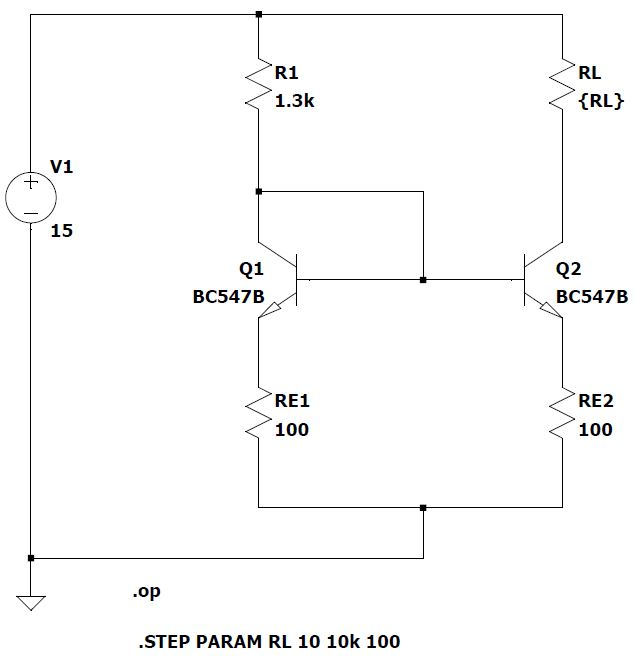
\includegraphics[width = 0.6\textwidth]{\figpath/einfacherStromspiegel.jpg}
    \caption{Einfacher Stromspiegel in LTSpice}
    \label{fig_Kap4_02:SpiceSchematic}
\end{figure}

Das Simulationsergebnis kann in Abb. \ref{fig_Kap4_03:Ia} betrachtet werden.

\begin{figure}[H]
	\centering \small
	\scalebox{0.9}{% This file was created by matlab2tikz.
%
\definecolor{mycolor1}{rgb}{0.00000,0.44700,0.74100}%
%
\begin{tikzpicture}

\begin{axis}[%
width=4.521in,
height=3.566in,
at={(0.758in,0.481in)},
scale only axis,
xmin=0,
xmax=10,
xlabel style={font=\color{white!15!black}},
xlabel={$R_L \text{ in k} \Omega$},
ymin=1,
ymax=11,
ylabel style={font=\color{white!15!black}},
ylabel={$I \text{ in mA}$},
axis background/.style={fill=white},
title style={font=\bfseries},
title={$I_a(R_L)$},
xmajorgrids,
ymajorgrids
]
\addplot [color=mycolor1, forget plot]
  table[row sep=crcr]{%
0.01	10.2021\\
0.11	10.19756\\
0.21	10.19295\\
0.31	10.18826\\
0.41	10.18349\\
0.51	10.17864\\
0.61	10.17371\\
0.71	10.16869\\
0.81	10.16358\\
0.91	10.15837\\
1.01	10.15307\\
1.11	10.14766\\
1.21	10.14216\\
1.31	10.13654\\
1.41	9.866105\\
1.51	9.252984\\
1.61	8.702559\\
1.71	8.211943\\
1.81	7.772927\\
1.91	7.378082\\
2.01	7.021202\\
2.11	6.697128\\
2.21	6.40157\\
2.31	6.130943\\
2.41	5.882232\\
2.51	5.652887\\
2.61	5.440736\\
2.71	5.243917\\
2.81	5.060831\\
2.91	4.89009\\
3.01	4.730487\\
3.11	4.580967\\
3.21	4.440606\\
3.31	4.308587\\
3.41	4.184188\\
3.51	4.066769\\
3.61	3.955759\\
3.71	3.850646\\
3.81	3.750974\\
3.91	3.65633\\
4.01	3.566343\\
4.11	3.480679\\
4.21	3.399033\\
4.31	3.321129\\
4.41	3.246716\\
4.51	3.175563\\
4.61	3.107462\\
4.71	3.04222\\
4.81	2.979661\\
4.91	2.919623\\
5.01	2.861956\\
5.11	2.806523\\
5.21	2.753197\\
5.31	2.701858\\
5.41	2.6524\\
5.51	2.604719\\
5.61	2.558722\\
5.71	2.514322\\
5.81	2.471435\\
5.91	2.429988\\
6.01	2.389907\\
6.11	2.351127\\
6.21	2.313586\\
6.31	2.277225\\
6.41	2.241988\\
6.51	2.207826\\
6.61	2.174689\\
6.71	2.142532\\
6.81	2.111312\\
6.91	2.080988\\
7.01	2.051524\\
7.11	2.022882\\
7.21	1.995029\\
7.31	1.967932\\
7.41	1.941562\\
7.51	1.915889\\
7.61	1.890886\\
7.71	1.866527\\
7.81	1.842788\\
7.91	1.819645\\
8.01	1.797076\\
8.11	1.77506\\
8.21	1.753577\\
8.31	1.732607\\
8.41	1.712134\\
8.51	1.692138\\
8.61	1.672604\\
8.71	1.653516\\
8.81	1.634859\\
8.91	1.616618\\
9.01	1.59878\\
9.11	1.581331\\
9.21	1.564258\\
9.31	1.547551\\
9.41	1.531196\\
9.51	1.515184\\
9.61	1.499503\\
9.71	1.484143\\
9.81	1.469095\\
9.91	1.454349\\
10	1.441328\\
};
\end{axis}
\end{tikzpicture}%}
	\caption{Ausgangsstrom in Abhängigkeit des Lastwiderstandes}
	\label{fig_Kap4_03:Ia}
\end{figure}

\section{Verlauf des Innenwiderstandes $R_i$}
Lt. Abb. \ref{} wird nun am Ausgang der Lastwiderstand durch eine Spannungsquelle ersetzt. 

\section{Temperaturabhängigkeit des Ausgangsstroms bei globaler Temperaturänderung}

\section{Temperaturabhängigkeit der Schaltung bei unterschiedlichen Bauteiltemperaturen}

\section{Vergleich mit Berechnung}